\usetikzlibrary{calc}
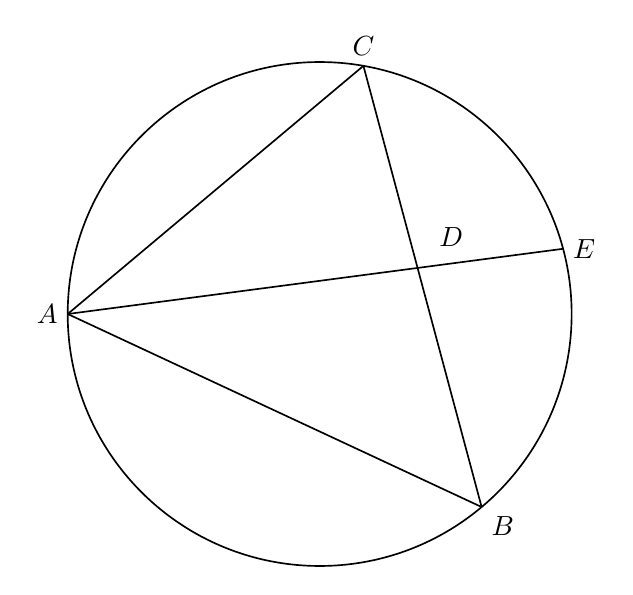
\begin{tikzpicture}[x=1cm,y=1cm,line width=.6pt,font=\normalsize]
\coordinate (O) at (0,0);
\coordinate (A) at (-3.2,0);
\coordinate (B) at (2.0569,-2.4513);
\coordinate (C) at (0.5557,3.1514);
\coordinate (E) at (3.091,0.8282);
\coordinate (D) at (1.2433,0.585);
\draw[black] (O) circle[radius=3.2cm];
\draw[black] (A)--(B);
\draw[black] (A)--(C);
\draw[black] (B)--(C);
\draw[black] (A)--(E);
\node[left] at (A) {$A$};
\node[below right] at (B) {$B$};
\node[above] at (C) {$C$};
\node[right] at (E) {$E$};
\node[above right,xshift=1.5mm,yshift=1.5mm] at (D) {$D$};
\end{tikzpicture}
